\documentclass[12pts]{article}

% pseudo Times New Roman
\usepackage{mathptmx}% http://ctan.org/pkg/mathptmx
% margins 1 in
\usepackage[a4paper, margin=1in]{geometry}
%line space
\renewcommand{\baselinestretch}{1.5}
% APA citations
\usepackage{apacite}
% math symbols
\usepackage{amssymb}
% tables created in rmd
\usepackage{longtable}
%math 
\usepackage{amsmath}
%images 
\usepackage{graphicx}
\usepackage{subcaption}

%opening
\title{QUANTAL RESPONSE EQUILIBRIUM IN A CITIZEN-CANDIDATE EXPERIMENT}
\author{Alexander Elbittar \and Andrei Gomberg \and Dario Trujano Ochoa}
\date{2018}

\begin{document}

\maketitle

\begin{abstract}

In this study, a Citizen-Candidate model of political competition was implemented in an experiment and the Quantal Response Equilibrium (QRE) was adjusted to data. 
This model of elections is based in the Hotelling-Downs model of spatial competition. 
However, candidates do not choose location, which in this case was their own ideal point, but to campaign or not. QRE is a generalization of the Nash equilibrium (NE) and player's responses are random. Six experimental conditions combine two entry cost levels, 
two voting systems (plurality rule and run-off), and three set of ideal points. 
The Nash Equilibrium (NE) is a good ex ante prediction in all games. 
Though, it cannot predict the large rate of participation nor the changes related to costs and ideal positions.  
In summary,  experimental  data  was explained  by QRE which assumes  a  stochastic  non-perfect  maximizing  decision rule when adjusted by game. However, in one game, the parameter that measures maximizing behavior was high compared with other games.


\end{abstract}

\section{Introduction}

    The citizen-candidate model (Osborne and Slivinski 1996, Besley and Coate 1997) is one of the few established approaches to endogenizing the number and the identity of political candidates and proposals in elections. In this environment a society of agents with publicly known preferences in some policy space has to decide on a common policy. Crucially, only alternatives explicitly proposed (nominated) by somebody shall be presented to voters and the nomination decision is strategic: citizens choose to nominate themselves, based on their predicted impact on the policy outcome, the cost of running for office and benefits accruing to office-holders. Once the set of candidates is fixed, the entire society votes and the elected candidate implements his/her favorite policy (as the individual preferences are public, candidates cannot commit to implementing any policy at variance with their ideal).
    Unfortunately, the citizen-candidate model is not easy to test using available electoral data, as it heavily relies on exact public knowledge of the the policy preferences of potential candidates, even those who may never be nominated in the actual election. Predictions of the model are, furthermore, dependent on parameters (such as the cost of running for office and the benefits of holding it) that might be difficult to measure empirically and even harder to exogenously vary in real political systems. A direct test of the model's prediction for the differential impact of different electoral systems is further complicated by the relative rarity of electoral system changes. The substantial multiplicity of equilibria for many parameter values in the model makes designing a satisfactory empirical test even harder.
    Many of the problems with testing the citizen-candidate model in the field can be overcome in an experimental lab. Thus, an experimentalist would have no difficulty varying office-holder benefits or nomination costs, changing the distribution of citizens in the policy space or even the electoral system. The hardest challenge is presented by the model's inherent equilbrium multiplicity for most "interesting" paramter values. Still, in the lab it is also possible to design environments that minimize this problem, allowing explicit tests of the model predictions.
    

    Surprisingly, in the more than twenty years since the publication of the original theoretical papers there has been little work on trying to test the model experimentally. The experimental literature on candidate behavior in elections has concentrated on candidate location decisions.
    <footnote>See, for instance, the early work by McKelvey and Ordeshook (1982) on two-candidate competition in environments with and without Condrocet winners, or a study by Aragonès and Palfrey (2004) on policy platform choice by candidates of different quality.
      
    However there has been comparatively little research on candidate entry. In fact, Palfrey (2016) in his survey of the field, noted that as of that moment he was aware of only two experimental studies concentrating on entry by policy-motivated candidates in this framework. Though an important advance, for being the first to attempt a laboratory testing of the model, Cadigan (2005) is somewhat limited in scope. It reports results of 2 treatments of an adaptation of the citizen-candidate model that are distinguished by the value of the cost of nomination parameter. In the high-cost treatment the unique predicted equilibrium involves a single candidate entering at the median of the voter distribution, while the low-cost treatment has, in addition to the median-candidate equilibrium, a two-candidate equilibrium with distinct policy proposals. The only other experimental test of the citizen-candidate environment that we are aware of has been conducted by ourselves (Elbittar and Gomberg, 2009). Unfortunately, the equilibrium multiplicity turned out to be a particularly serious problem in that stdy, resulting in major coordination problems among the subjects.
    
    Our objective in this work was to design an environment, which avoids the coordination problems, while varying both cost parameters and electoral systems. In particular, in addition to the simple plurality elections, we consider the two-round runoffs. In particular, Osborne and Slivinski (1996) results imply, for certain parameter values of the model, a stronger pull for entry by politicians at the median of the voter ideal point distributions. The same pull to the center is implied by high candidate entry cost for both electoral systems. It is these implications of the model that we would like to test.
    
    Like both Cadigan (2005) and Elbittar and Gomberg (2009), we impose sincere voting, in order to concentrate on individual entry decisions by potential candidates. At the same time, we want to stay close to the large-electorate spatial model of Osborne and Slivinski (1996). To do this, while keeping the number of participants in an experimental game small, we decouple the potential candidates (whom we shall call "politicians") from the entire society of citizens. Only politicians may choose to run for office, while the set of voters (implemented in our experiments by a computer) is larger. In practice, not every voter would have name recognition and/or funding lined up to make him a viable candidate in a given election, Furthermore, only politicians are under a sufficient public scrutiny to make the assumption that their political views are known empirically plausible. In most elections, at least some of the potential "pre-candidates", though credible enough to be considered, choose not to enter the campaign. It is this entry decision that we study.
    
    Cadigan (2005) observed that the low-cost treatment results in relatively high entry by symmetric off-median subjects, compared with the high-cost treatment.  Furthermore, he notes non-negligible entry rates by candidates who, according to the model predictions, should not enter. This might seem unexpected, given that in related games of market entry, which have been extensively studied experimentally since Kahneman (1988), fast convergence to theoretically predicted entry rates of entry has been commonly observed (for a survey, see, for instance, Camerer 2003). However, Rapoport et al. (2002),in a market-entry game with asymmetric entry costs, found that subjects tend to over-enter, when the pure-strategy equilibrium implies they should be staying out, and under-enter, when the equilibrium implies they should enter. Unlike in Rappoport et al. (2002) in the citizen-candidate environment the candidate asymmetry comes not from difference in entry costs, but from a difference in their spatial location. Still, a parallel seems notable.
    
    Our own earlier obervations in Elbittar and Gomberg (2009) may be summarized as follows. Firstly, we do observe subjects reacting to treatment variable changes. In particular, both the asymmetry of politician ideal point distribution and the run-off electoral system are conducive to greater entry frequencies at the median of the voter ideal points. Secondly, we seem to confirm Cadigan's observation of comparatively high entry in situations, when equilibrium predicts no entry. In fact, entry rates remain non-negligible even from, essentially, hopeless positions. Other than that, the subjects' entry decisions seem to be reasonably close to best responding to the empirically observed entry frequencies.

The Rest of this paper is organized as follows. Section 2 presents the basic citizen-candidate model along the lines of Osborne and Slivinski (1996), section 3 describes the experimental design we emply, section 4 presents our experimental results, including the quantal response equilibrium analysis, section 5 concludes.






\section{Model}

%The Citizen-Candidate (Osborne and Slivinski 1996) model of political competition is described in detail.
Our model adapts the one originally introduced in Osborne and Slivinski (1996). While Besley and Coate (1997) provide a similar model which allows for a small number of agents (a setting which would seem to be easier to implement in a lab), we follow the Osborne and Slivinski approach, as we are interested in large elections, where voting may be assumed to be non-strategic (allowing for strategic voting would introduce additional equilibrium multiplicity which we are trying to avoid). In addition, like in Osborne and Slivinski (1996), we concentrate on the comparison of candidate entry under distinct voting rules.

We consider a society that has to implement a single policy\ $x$ on a
unidimensional $\left[ 0,100\right] $ continuum. Heterogenous voters have
single-peaked preferences, with ideal points distributed over the continuum
according to some distribution $F$ (for the rest of the paper it shall be assumed to be uniform). Our main
departure from Osborne and Slivinski is in limiting the set of possible
candidates to a small finite subset of citizens with corresponding ideal points 
\(Q=\{q_1, ..., q_n\}, q_i \in \left[ 0,100\right]\). 

Potential candidates, or politicians, may choose to
nominate or not to nominate themselves for the office. As in Osborne and Slivinski (1996) it is assumed that agent preferences are known by everyone and that there is no commitment, so
that the politicians can only promise that if elected they would implement
their ideal policies. The rest of the
voters are assumed to never run for the office, but simply to vote for the
candidate whose ideal policy is the closest to their own (in experimental
treatments we shall automate this part of the set-up). 

Hence, the game has $N=\left\{ 1,2,....n\right\} $ politician
players. Each player $i$ has a 2-point strategy space $S_{i}=\left\{
0,1\right\} $, where $s_{i}=1$ means the agent nominates him/herself, and $%
s_{i}=0$ means the agent stays out of the election. Potential candidates consider the cost of participation $c$, the
possible benefits of being elected or "ego rent" $b$, and the distance between their ideal policy and the final policy implemented. As in Osborne and Slivinsky (1996) we assume that if everybody decides not to enter the resultant outcome is "catastrophic": a large negative payoff $-D$ for everyone. To summarize, individual payoff in this game is given by  \ref{eq:Utility} represent the preferences of citizens:

\begin{equation}
u_i(x,q_i)=
\begin{cases}
-D, & \text{if } s_i=0, \forall i \in Q \\
-\alpha||x-q_i|| - cs_i + bw_i(s), & \text{otherwise} 
\end{cases}\label{eq:Utility}
\end{equation}

where $\alpha$ is a parameter reflecting the relative importance of policy vis-a-vis non-policy payoffs and $w_i$ takes value of $1$ if the agent wins and $0$ otherwise. Notice, that whether a candidate wins depends on the voting system, voter ideal point distribution, and the profile of individual entry decisions $\(s=\{q_1, ..., q_n\})$.

Unlike the politicians, who have a strategic role to play, regular voters in our experiment will becomputerized robots, who always vote sincerely. We assume there are 101 such
voters, with a single voter having an ideal point at every integer between $
0 $ and $100$ (we chose to use a discrete voter space in order
to avoid explaining the notion of a continuous distribution to subjects who were, for the most part, not exposed to calculus or probability theory). The robot voters always vote for a
nominated candidate whose ideal point is closest to their own (in case $m>1$
candidates are at the same distance from a given voter, s/he shall randomly
select a candidate, with every one of the closest candidates having a
probability $\frac{1}{m}$ of being chosens).

The winner of the election is determined by the voting of a larger society.
In this paper we consider two voting rules:

\begin{itemize}
	\item \textbf{Simple Plurality}:
The candidate who gets most votes wins, with ties resolved randomly, with every one of the leading candidates having equal probability of winning. 
	
	\item \textbf{Runoff}:
	The two candidates with highest votes from a first round are presented for the same set of voters to choose from in the second round, in which the winner is determined as in the plurality rule and ties in both rounds resolved randomly, with equal probability of being chosen among the tied candidates.
\end{itemize}

Following the bulk of the earlier literature, we shall concentrate on the pure strategy Nash equilibria. An important role in our setting shall be played by the distance between the politician ideal points and the meidan of the voter distribution $m$.  The following
proposition, which follows from the results of Osborne and Slivinski (1996),
describes some of the equilibrium possibilities in our setting. It is these
implications of the model that we shall try to test in the lab.

\begin{proposition}
	a) If there is a unique politician closest to , then for both voting
	rules there exists an equilibrium in which he is the only candidate.
	
	b) In every two-candidate equilibrium under the plurality rule the
	candidates are located symmetrically around $m$. Furthermore, such an equilibrium will exist only if there are symmetric politicians located close enough to $m$ , or if the symmetric
	politicians are the closest ones to $m$.
	
	c) If there are exactly two potential candidates closest to $m$, then under
	the run-off system there exists an equilibrium in which they are the only
	entrants if only if $2c\leq b$.
	
\end{proposition}



\section{Experimental Design and Predictions}

All experimental sessions were conducted at the Instituto Tecnologico Autonomo de Mexico (ITAM) 
in Mexico City and the subjects were undergraduates recruited in introductory economics courses. 
The experiments were computer-administered. A total of 10 experimental sessions were conducted 
and each session had between 12 and 30 participants.

In each experimental session we consecutively ran 30 elections in groups with
three candidates, with both group membership and subject ideal points
randomly changed before each election. If the total number of subjects in the
room was not divisible by 3, in each round some subjects would
be randomly selected to sit it out. Therefore, up until the last round the termination
time effectively remained random. At the beginning of each session, subjects played three practice trials.

The distribution of subjects ideal points was either constant, or varied only
once during a session, but each subject?s location was randomly chosen for each
period, which corresponded to an election. In each election subjects, having
observed their positions, had to decide whether to nominate themselves as possible
candidates. All voter decisions were taken by the computer. After each election
subjects got the feedback about the ideal points of the entrants and the
winner in their election, as well as the vote shares received by every candidate
and their own monetary payoff.

Less trials happened if participants lost all the money given or because there were a non-multiple of three; 
then, one or two participants waited until the next trial-match. 
All payments were in Mexican Pesos (MN$11 = USD$1). We started each experimental
session by allocating every agent MN140 pesos of initial capital, to
which the payments corresponding to the model parameter values were added
and subtracted. Participants were allowed to continue until 
they finished a trial with negative balance.

All six experimental treatments had three candidates with different ideal points from the interval $[0, 100]$ 
which represents the sincere voters. The six different games were built from 2 entry costs, 
2 voting rules and 3 ideal points sets. Table \ref{tab:parameters} summarizes each game parameters. 
The last three columns show the ideal points labeled \emph{Left}, \emph{Center} and \emph{Right} according 
with the relative position held by each candidate. The last four game have the same ideal position and were 
built from crossing costs $5$ and $20$ with the two voting rules. 

\begin{table}[!htbp] \centering 
	\caption{Parameters in the six treatments} 
	\label{tab:parameters} 
	\begin{tabular}{@{\extracolsep{5pt}} ccccccccc} 
		\\[-1.8ex]\hline 
		\hline \\[-1.8ex] 
		Games & VotingRule & $\alpha$ & $c$ & $b$ & $D$ & Left & Center & Right \\ 
		\hline \\[-1.8ex] 
		PLCS & Plurality Rule & $0.100$ & $5$ & $25$ & $40$ & $30$ & $50$ & $70$ \\ 
		PLCA & Plurality Rule & $0.100$ & $5$ & $25$ & $40$ & $30$ & $50$ & $80$ \\ 
		PL & Plurality Rule & $0.100$ & $5$ & $25$ & $40$ & $20$ & $30$ & $80$ \\ 
		PH & Plurality Rule & $0.100$ & $20$ & $25$ & $40$ & $20$ & $30$ & $80$ \\ 
		RL & Run-Off & $0.100$ & $5$ & $25$ & $40$ & $20$ & $30$ & $80$ \\ 
		RH & Run-Off & $0.100$ & $20$ & $25$ & $40$ & $20$ & $30$ & $80$ \\ 
		\hline \\[-1.8ex] 
	\end{tabular} 
\end{table} 


The Nash equilibria in pure strategies are stated in table \ref{tab:equilibria}. The only games with two-candidate equilibrium are \emph{PLCS} and \emph{PL}, which are those with low cost, extreme ideal points symmetric around median and voting  plurality rule. The closest equilibrium to empirical proportion of entering are marked with an asterisk. 

\begin{table}[!htbp] \centering 
	\caption{Possible equilibria with the ideal points of entering candidates}
	\label{tab:equilibria} 
	\begin{tabular}{@{\extracolsep{5pt}} ccc} 
		\\[-1.8ex]\hline 
		\hline \\[-1.8ex] 
		Games & OneCandidate & TwoCandidate \\ 
		\hline \\[-1.8ex] 
		
		PL & \textbf{30*} & $20$, $80$ \\ 
		PH & \textbf{30*} &  \\ 
		RL & \textbf{30*} &  \\ 
		RH & \textbf{30*} &  \\ 
		PLCS & $50$ & \textbf{30*, 70*} \\ 
		PLCA & \textbf{50*} &  \\ 
		\hline \\[-1.8ex] 
	\end{tabular} 
\end{table} 



\section{Results}


\begin{table}[!htbp] \centering 
  \caption{Characteritics by Sessions} 
  \label{tab:sessions} 
\begin{tabular}{@{\extracolsep{5pt}} cccc} 
\\[-1.8ex]\hline 
\hline \\[-1.8ex] 
Juego & Sesion & No.Participants & Bankrupcy \\ 
\hline \\[-1.8ex] 
PLCS/PLCA & $1$ & $18$ & $0$ \\ 
PLCS/PLCA & $2$ & $15$ & $0$ \\ 
PLCA/PLCS & $1$ & $21$ & $1$ \\ 
PLCA/PLCS & $2$ & $12$ & $0$ \\ 
PL & $1$ & $19$ & $0$ \\ 
PL & $2$ & $18$ & $0$ \\ 
PL & $3$ & $20$ & $0$ \\ 
PH & $1$ & $15$ & $9$ \\ 
PH & $2$ & $20$ & $13$ \\ 
PH & $3$ & $23$ & $16$ \\ 
RL & $1$ & $26$ & $0$ \\ 
RL & $2$ & $16$ & $0$ \\ 
RL & $3$ & $27$ & $2$ \\ 
RH & $1$ & $15$ & $4$ \\ 
RH & $2$ & $15$ & $5$ \\ 
RH & $3$ & $15$ & $6$ \\ 
\hline \\[-1.8ex] 
\end{tabular} 
\end{table} 


A summary of experimental sessions is presented in table \ref{tab:sessions}. All the treatments had three sessions, except for $PLCS$ and $PLCA$ which had only two sessions. In table \ref{tab:rawentry},  we can see the total number of entries in each game by each ideal position. The differences among the number of total trials is due to bankruptcy of the participants that could not longer play.


\begin{table}[!htbp] \centering 
  \caption{Total number of entries by position and game} 
  \label{tab:rawentry} 
\begin{tabular}{@{\extracolsep{5pt}} ccccccc} 
\\[-1.8ex]\hline 
\hline \\[-1.8ex] 
Position & PL & PH & RL & RH & PLCS & PLCA \\ 
\hline \\[-1.8ex] 
Left & 254 &  89 & 254 &  82 & 296 & 299 \\ 
\% & (47) & (23.4) & (39.2) & (23.4) & (89.7) & (90.6) \\ 
Center & 468 & 332 & 630 & 337 & 164 & 263 \\ 
\% & (86.7) & (87.4) & (97.2) & (96.3) & (49.7) & (79.7) \\ 
Right & 468 & 218 & 278 &  82 & 297 & 164 \\ 
\% & (86.7) & (57.4) & (42.9) & (23.4) & (90) & (49.7) \\ 
Total & 540 & 380 & 648 & 350 & 330 & 330 \\ 
\hline \\[-1.8ex] 
\end{tabular} 
\end{table} 


\begin{figure}
	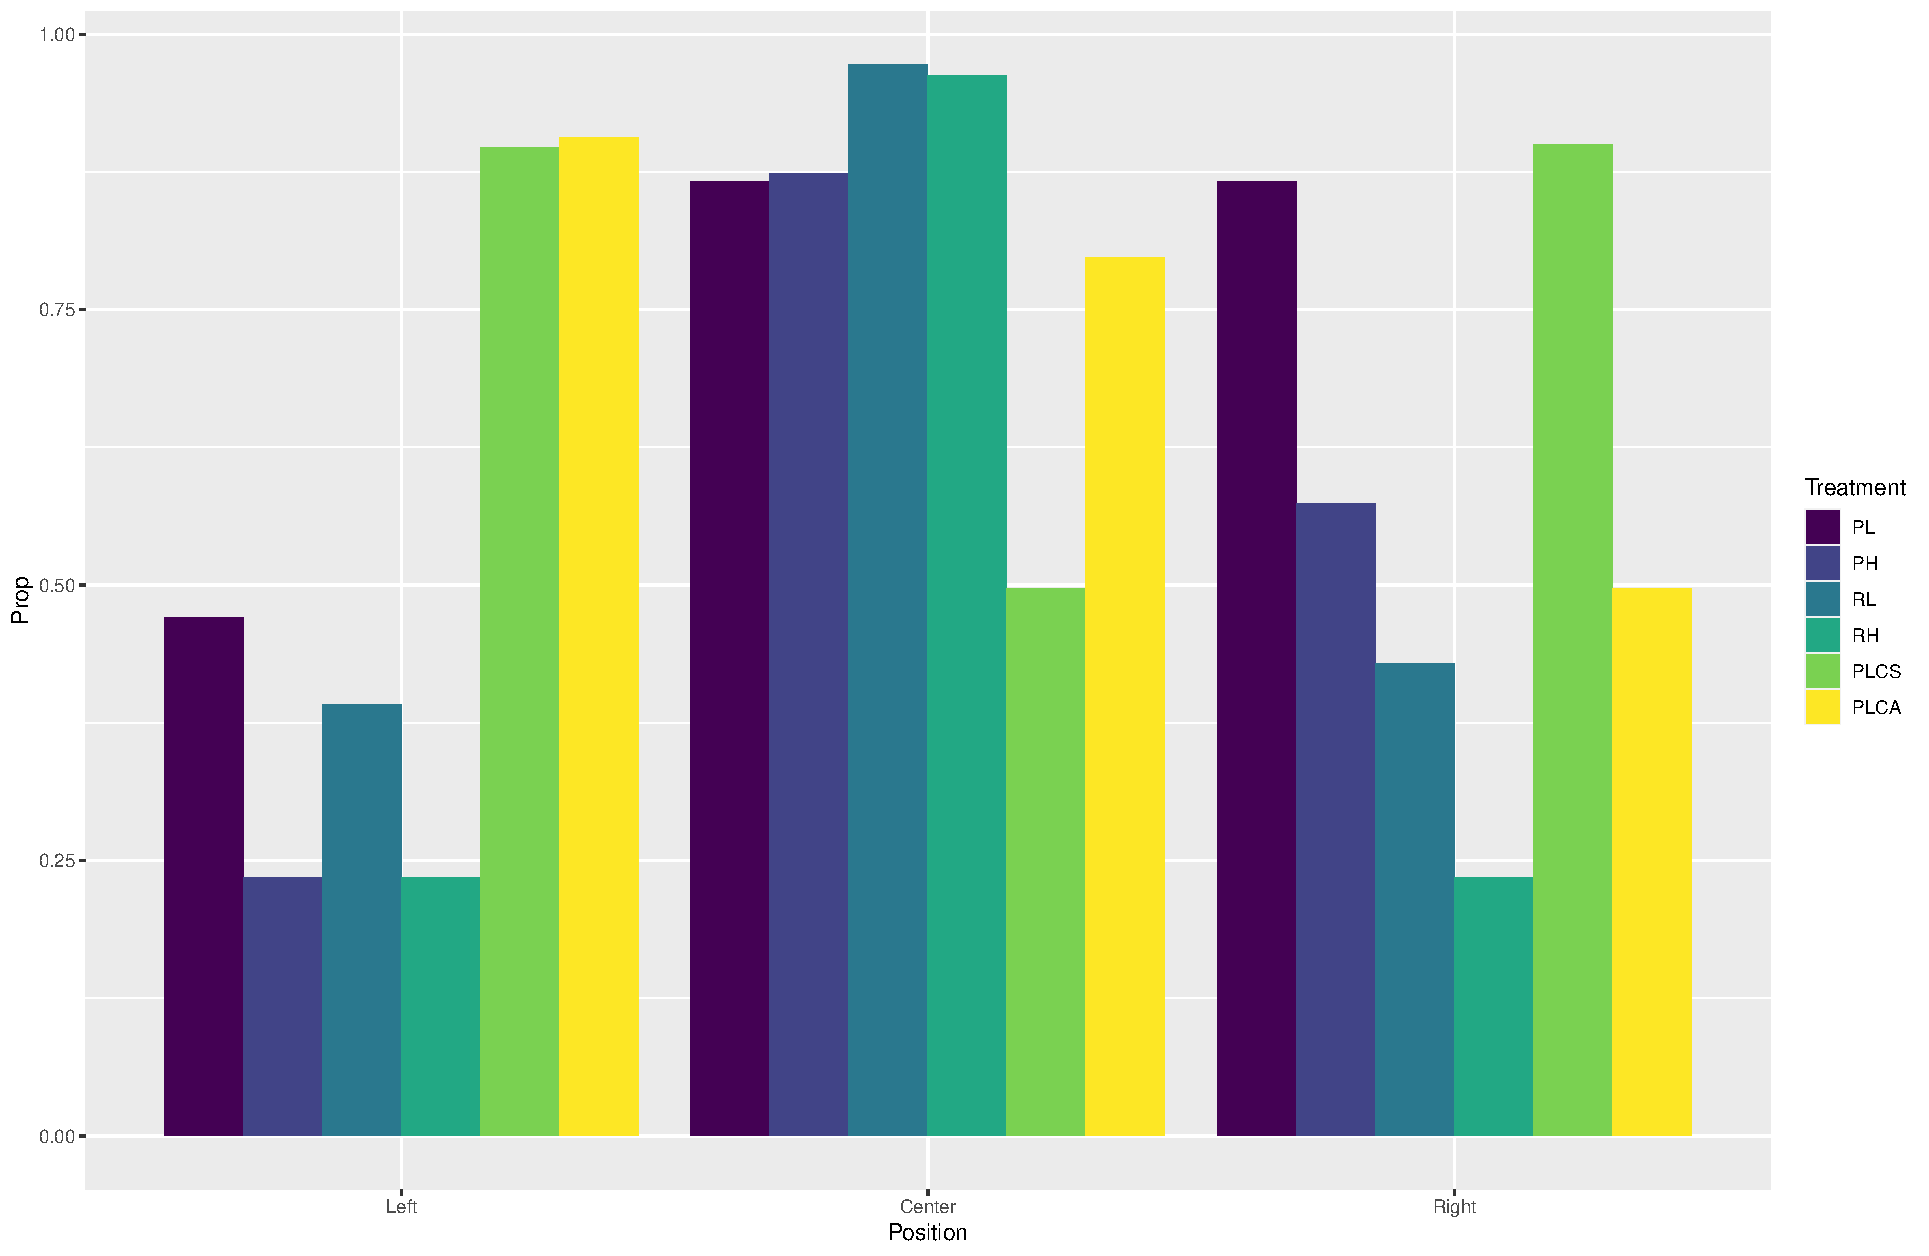
\includegraphics[width=1\linewidth, height=7cm]{../../results/figures/barplot_prop} 
	\caption{Barplot}
	\label{fig:barplot}
\end{figure}

\begin{figure}
	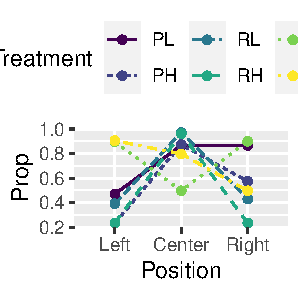
\includegraphics[width=1\linewidth, height=7cm]{../../results/figures/lines_prop} 
	\caption{Lines}
	\label{fig:lines}
\end{figure}


\subsection{Distribution of Errors}

Considering how people behave, it is possible to measure the error as the difference between what participants should have done (choose the option with the highest expected payoff) and what they did (proportion of entry). Then, considering the proportion of entry, a negative value means that they enter less than what is optimal, and a positive value means that they over-participate when they should not. In figure \ref{fig:errordist}, it can be seen the distribution of such error by game and position.


\begin{figure}[h]
	
	\begin{subfigure}{0.5\textwidth}
		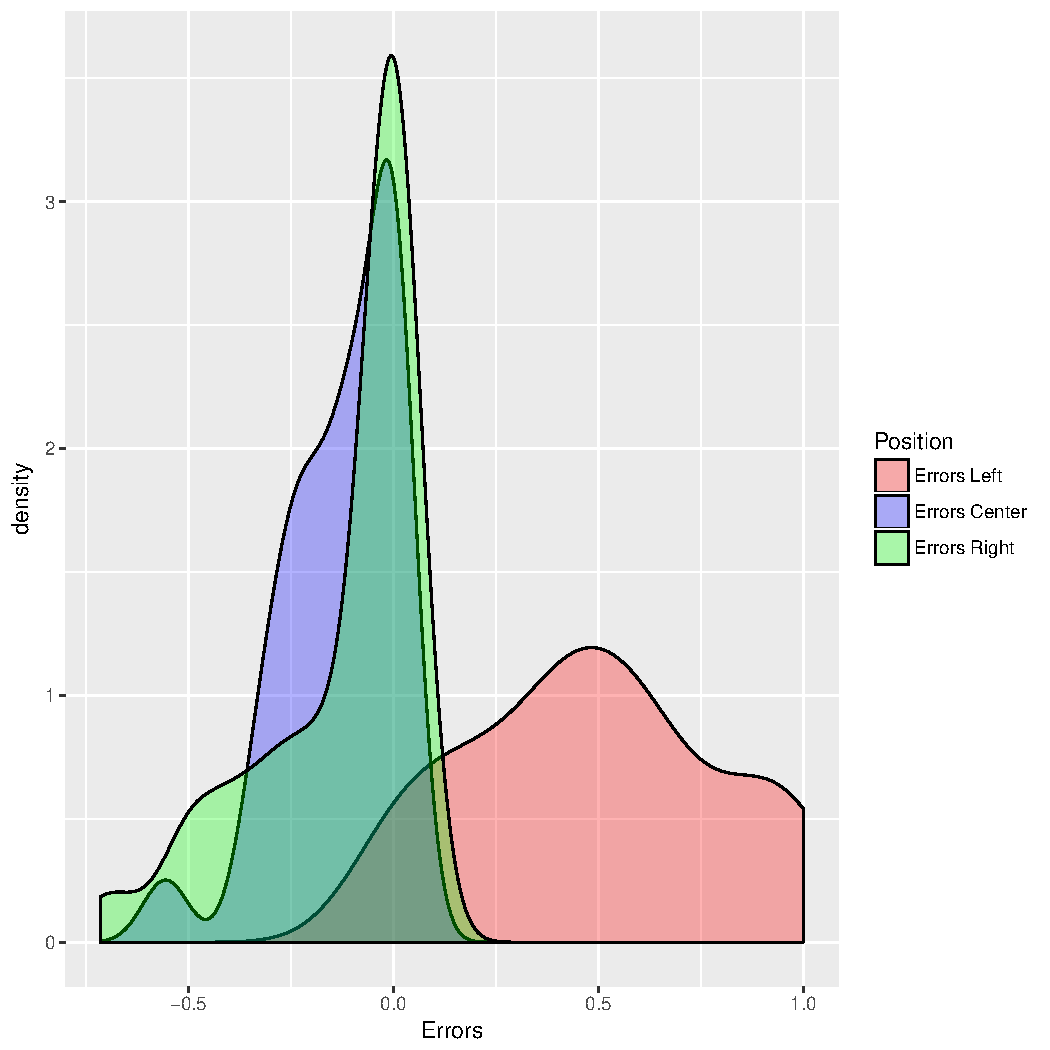
\includegraphics[width=1\linewidth, height=7cm]{../../results/figures/errorDistributionPR_LC} 
		\caption{PR\_LC}
		\label{fig:errdistsubim1}
	\end{subfigure}
	\begin{subfigure}{0.5\textwidth}
		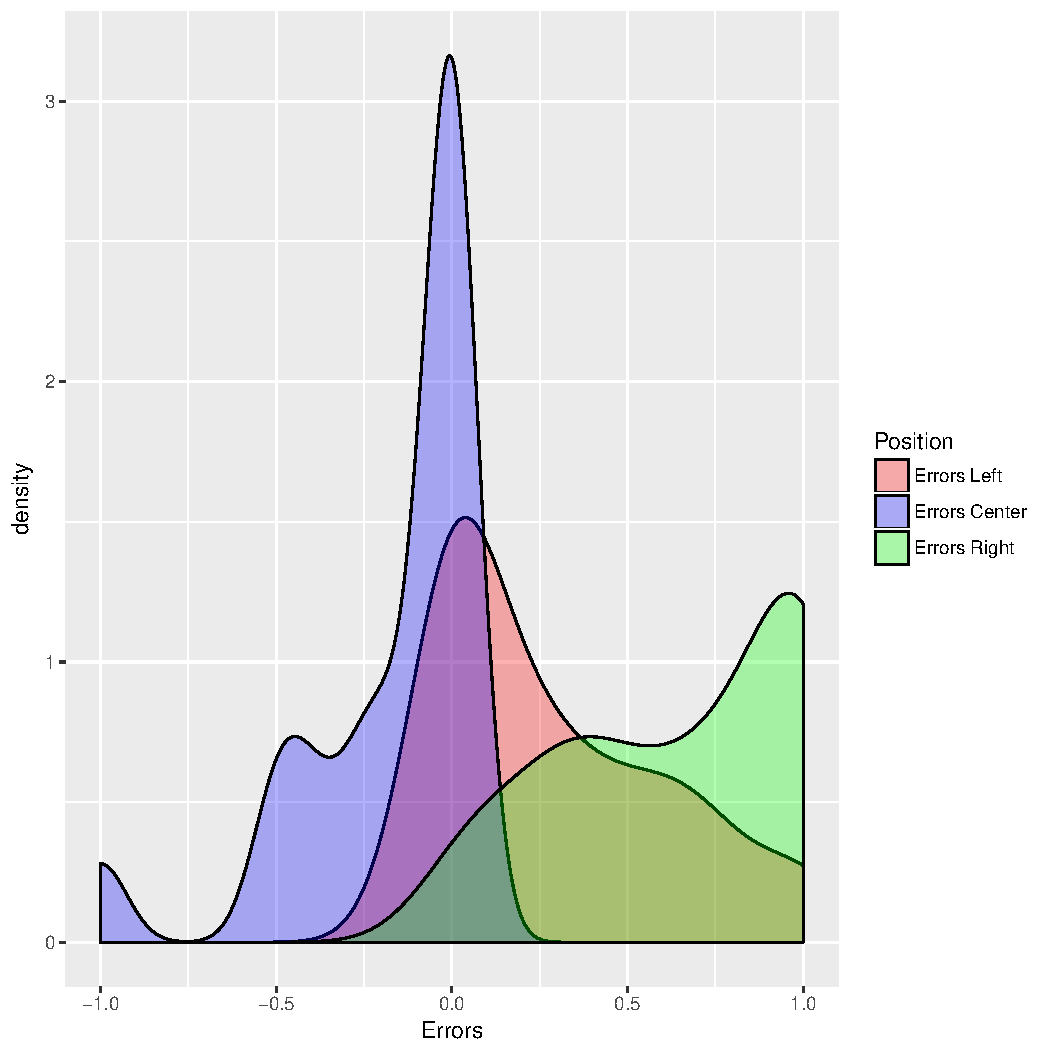
\includegraphics[width=1\linewidth, height=7cm]{../../results/figures/errorDistributionPR_HC}
		\caption{PR\_HC}
		\label{fig:errdistsubim2}
	\end{subfigure}

	\begin{subfigure}{0.5\textwidth}
	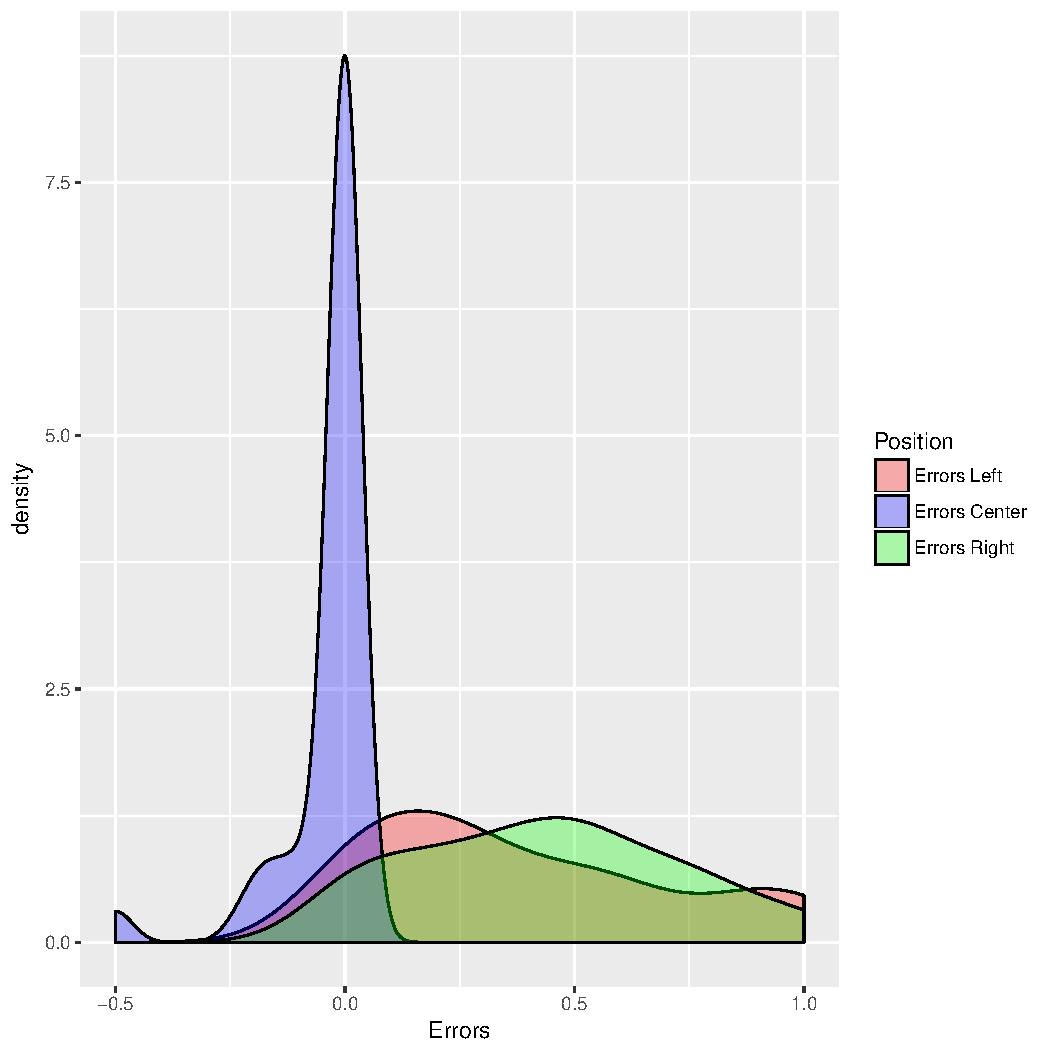
\includegraphics[width=1\linewidth, height=6cm]{../../results/figures/errorDistributionRO_LC} 
	\caption{RO\_LC}
	\label{fig:errdistsubim3}
	\end{subfigure}
	\begin{subfigure}{0.5\textwidth}
	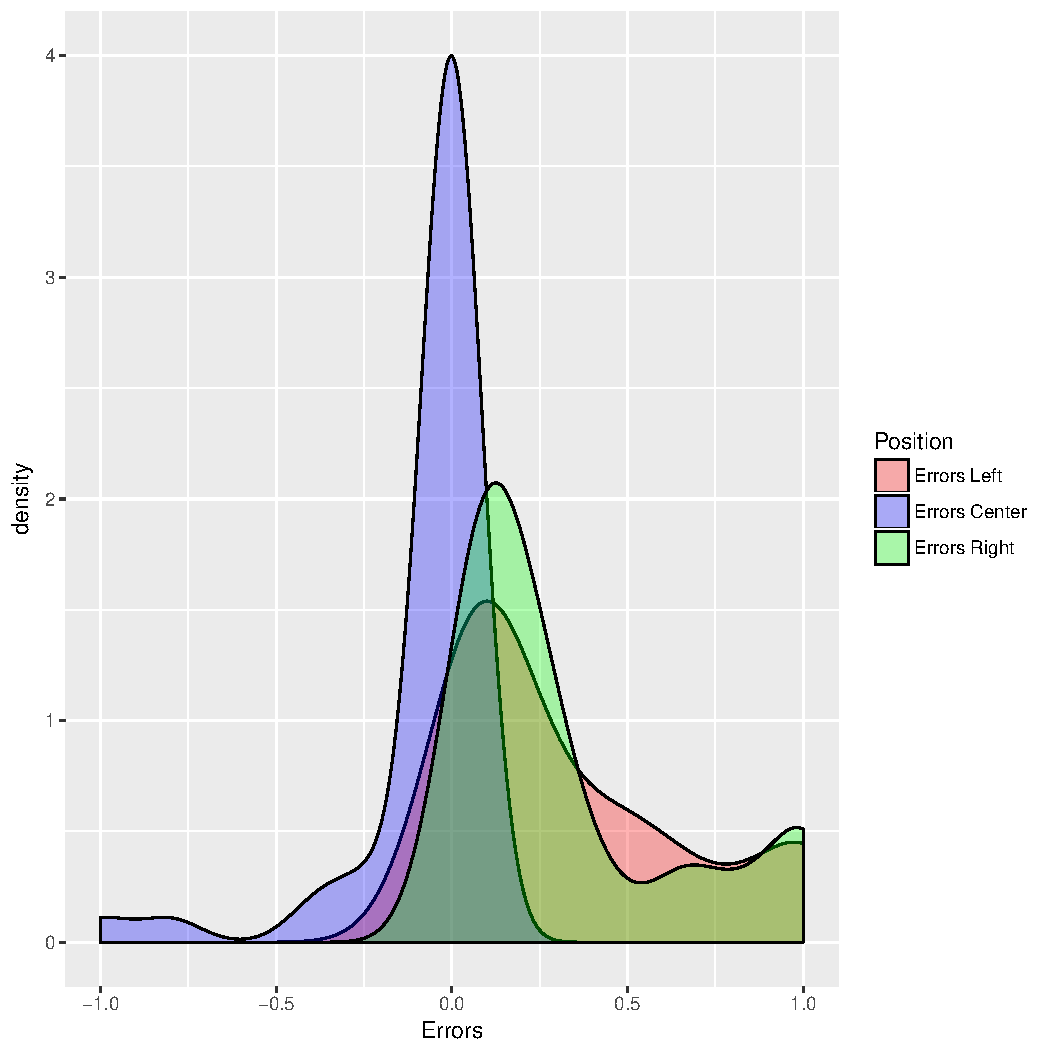
\includegraphics[width=1\linewidth, height=7cm]{../../results/figures/errorDistributionRO_HC}
	\caption{RO\_HC}
	\label{fig:errdistsubim4}
	\end{subfigure}

	\begin{subfigure}{0.5\textwidth}
	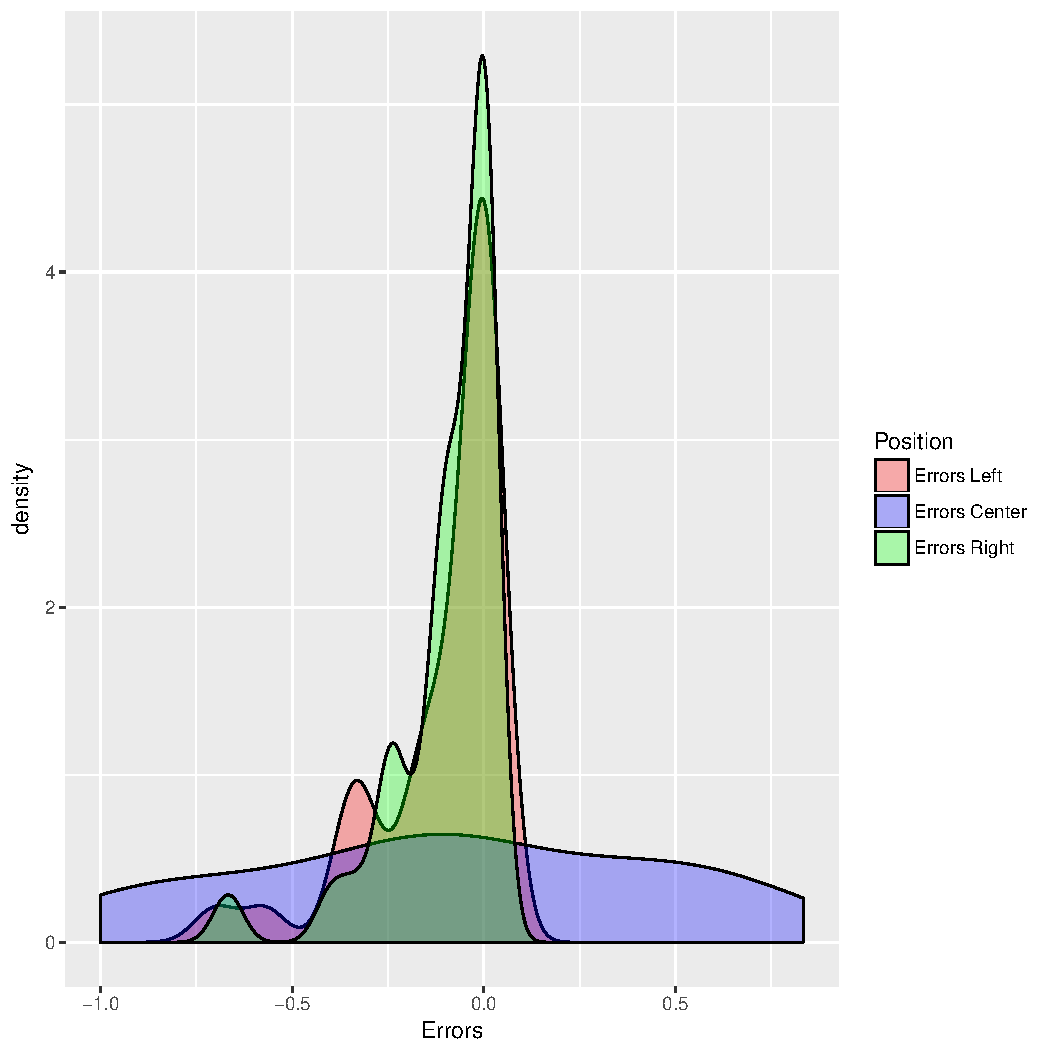
\includegraphics[width=1\linewidth, height=7cm]{../../results/figures/errorDistributionex70} 
	\caption{ex70}
	\label{fig:errdistsubim5}
	\end{subfigure}
	\begin{subfigure}{0.5\textwidth}
	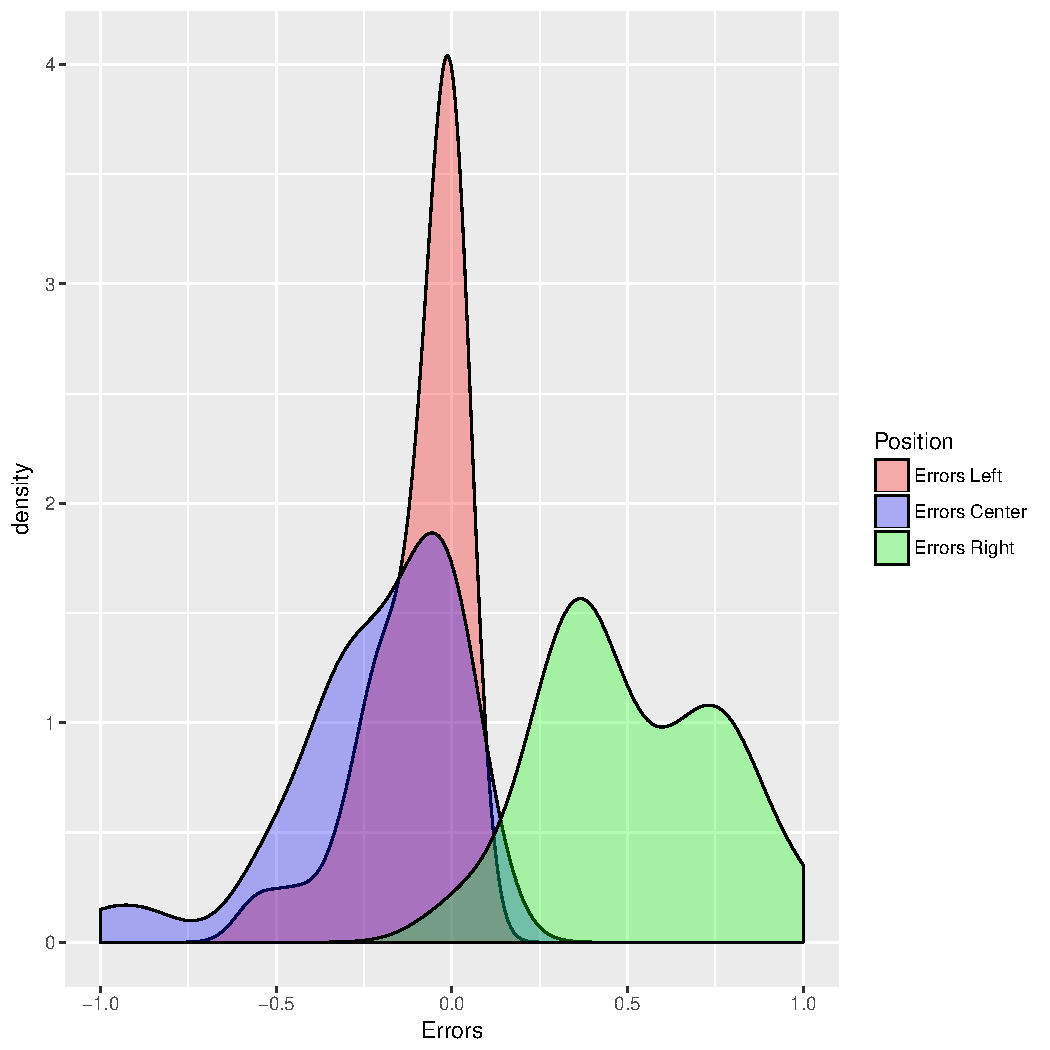
\includegraphics[width=1\linewidth, height=7cm]{../../results/figures/errorDistributionex80}
	\caption{ex80}
	\label{fig:errdistsubim6}
	\end{subfigure}
	
	\caption{Distribution of error by game and position. For each participant, the error was calculated as the difference between the proportion of entry observed and the optimal entry according with the expected payoff calculated based on the entry proportion of all participants in the session.}
	\label{fig:errordist}
\end{figure}


Participants in the central position do not deviate too much from the optimal decision. It is particularly clear in the games whit the same ideal positions $Q=\{20, 30, 80\}$. However, as can be seen in the graph \ref{fig:errdistsubim5}, the behavior in this position is completely random in the game \emph{ex70}, where the extreme positions enter frequently. Furthermore, players in these positions make less mistakes. On the other hand, errors are biased towards over-entering, with some exceptions among participants in the central position. Particularly, in games \emph{PR\_LC} an d\emph{ex80} there is a clear recognition of the over-entering position (figures \ref{fig:errdistsubim1} and \ref{fig:errdistsubim6}). In both cases, that position is the closest to the winning central. This could be due to the fact that, in terms of payoffs, they did not lose too much if the central position wins, but still they continue participating. 

% lets change names

\section{QRE}

The Quantal Response Equilibrium (QRE) proposed by (Richard D McKelvey
and Palfrey 1995) is constructed on the base of a stochastic best
response function. The most used implementation is the logistic function
over the difference between the expected payoff of the options:

\begin{equation}\label{fn:SBR}
\sigma_{ij}= \displaystyle\frac{e^{(\pi_{j})\lambda}}{e^{(\pi_{j})\lambda}+e^{(\pi_{i\ne j})\lambda} } 
=\displaystyle\frac{1}{1+e^{(\pi_{i\ne j}-\pi_{j})\lambda }}        
\end{equation}

The degree of stochasticity in the electionis determined by \(\lambda\). When
\(\lambda \rightarrow 0\) the election is a fair coin tossing for each
option independent of the expected payoffs (minimum level of
rationality), and when \(\lambda \rightarrow \infty\) the election is
deterministic with the more profitable action being chosen with
certainty (complete rationality). The expected payoff of action \(j\) is
represented by \(\pi_j\). Notice that $\pi_j: \sigma_{-i} \rightarrow \mathbb{R}$, where $\sigma_{-i}$ stands for others' distribution of probability.

An easy way to visualize the effect of \(\lambda\) over decisions is to
remember the logistic regression: the dependent variable is the
probability to choose option \(j\), and the independent variable is the
difference between expected payoffs of the two options. Intercept is
fixed in zero -which imply equal probability when options' expected
payoffs are the same-, and slope is precisely \(\lambda\), what
determines how step is the logistic function. For this reason,
\(\lambda\) is also interpreted as the level of rationality: as it
increases, decision will be better in terms of expected payoffs and less
uncertain.


With equation \ref{fn:SBR} a stochastic best response is defined:

\begin{equation}
\sigma^*_{ij}(\lambda, \beta, \pi_{j}(\sigma_{-i}))
\end{equation}\label{eq:SBR} 

, which is the player \(i\)'s probability of choose the
actions \(j\) (i.e.~Entry or Not Entry in the Citizen-Candidate model).
Vector \(\beta\) commonly refers to economic parameters that can measure
risk aversion or altruism. In the present analysis, I do not consider
these possibilities, but because \(\beta\) refers to changes in the
original payoff matrix, I will use \(\beta\) to refer to different
games.

With equation \ref{eq:SBR}, a distribution over actions for each player
is defined: \[\sigma^*_{i}(\lambda, \beta, \sigma_{-i})\]

This stochastic best response have the proprieties of a regular quantal
response function stated by (Goeree, Holt, and Palfrey 2016):

\begin{itemize}
	\item Interiority: $\sigma_{ij} >0$
	\item Continuity: $\sigma_{ij}$ is continuous and differentiable. 
	\item Responsiveness:  $\partial \sigma_{ij} / \partial \pi_{ij} >0 $
	\item Monotonicity: $\pi_{ij}> \pi_{ik} \Rightarrow \sigma_{ij}>\sigma_{ik}$
\end{itemize}

Notice that stochastic best response is a function of others' mixed
strategies (\(\sigma_{-i}\)). This is the case because, as seen in
equation \ref{fn:SBR}, probability depends on \(\pi_{j}\) which is a
function of others' strategies: \(\pi_{j}(\sigma_{-i})\). In the case of
the Citizen-Candidate model, \(\pi_j\) is the expected payoff of
equation \ref{eq:EU}.

Define then the function:

\begin{equation}\label{eq:sigma}
\sigma = (\sigma^*_{1}, ..., \sigma^*_{N})
\end{equation}

Then, quantal response equilibrium (\(\sigma^*\)) is a fixed point of
equation \ref{eq:sigma}, that now is a function only of \(\lambda\) and
\(\beta\). Due to the proprieties of the stochastic best response, and
using the fixed point theorem, the equilibrium existence is assured.
The QRE can be seen as the solution of a non-linear system of equations which is solved numerically. 

Note that a different equilibrium is predicted depending of the value of
\(\lambda\) and that players tend towards pure strategies as \(\lambda\)
goes larger. This equilibrium is called logit equilibrium (Goeree, Holt,
and Palfrey 2016). The software Gambit (Richard D. McKelvey, McLennan,
and Turocy 2014) allows to see those equilibria as a function of the
rationality parameter \(\lambda\). I realized the calculus in \emph{R}
(R Core Team 2017) with the package \emph{nleqslv} (Hasselman 2017), and
compare the result with gambit's; they are the same.

\subsection{Maximul Likelihood Estimation of $\lambda$}

Data analysis at different levels was calculated by maximum likelihood,
following directions from (Goeree, Holt, and Palfrey 2016). The
equilibrium correspondence approach was used: the QRE is calculated for
a given \(\lambda\) and other parameters (\(\beta\)):
\(\sigma*_{ij}(\lambda, \beta)\). In order to find this function, a non
linear equations system with no analytical solution has to be solved.
This was done using the R package \emph{nleqslv} (Hasselman 2017).

Once this function is constructed, it is possible to find the general
logLikelihood objective function, and the then optimize it.

\begin{equation}\label{fn:MLE}
logL(\lambda) = 
\Sigma^n_{i=1} \Sigma^{J_i}_{j=1} f_{i,j} log(\sigma^*_{ij}(\lambda, \beta))
\end{equation}

In the objective function \ref{fn:MLE}: \(n=3\), \(J_i = 2\) and
\(f_{i,j}\) are the times each i-th citizen choose their j-th option. Notice that it was constructed under the assumption of independence of decisions. Also it is assumed that $\lambda$ is the same for all of them.
The Global and by game estimators are in table \ref{tab:mle}.

\begin{table}[!htbp] \centering 
	\caption{} 
	\label{} 
	\begin{tabular}{@{\extracolsep{5pt}} cccccccc} 
		\\[-1.8ex]\hline 
		\hline \\[-1.8ex] 
		X & Global & PR\_LC & PR\_HC & RO\_LC & RO\_HC & ex70 & ex80 \\ 
		\hline \\[-1.8ex] 
		Estimate & $0.078$ & $0.084$ & $0.072$ & $0.098$ & $0.083$ & $0.222$ & $0.075$ \\ 
		sd & $0.001$ & $0.003$ & $0.001$ & $0.004$ & $0.002$ & $0.007$ & $0.004$ \\ 
		\hline \\[-1.8ex] 
	\end{tabular}\label{tab:mle}
\end{table} 

QRE estimation is a punctual number, but the graph of $\sigma (\lambda, \beta)$ can be built for each game. Figure \ref{fig:QRE} displays such function. We can see that when $\lambda=0$ all the players choose entry with $0.5$ probability, and how they approach smoothly towards a some NE. Also, we can see how well the model explain data. Horizontal lines, with their colors corresponding with each player, are the observed proportion in the experiment. Solid vertical line is the global estimate of $\lambda$, and dotted line is the estimation within each game. Where those lines cross is the QRE prediction.

In general, the value of $\lambda$ is similar among games, except for \textit{ex70} game. The estimated is too large compared with the other games, even when it can be seen that prediction is almost perfect. The reasons for this divergence must be investigated more deeply. The worst adjustment is in the \textit{ex80} game where $q_{30}$'s observed proportion of entry is higher than $q_{50}$'s, a fact that QRE cannot explain.

\begin{figure}
	\begin{subfigure}{0.6\textwidth}
		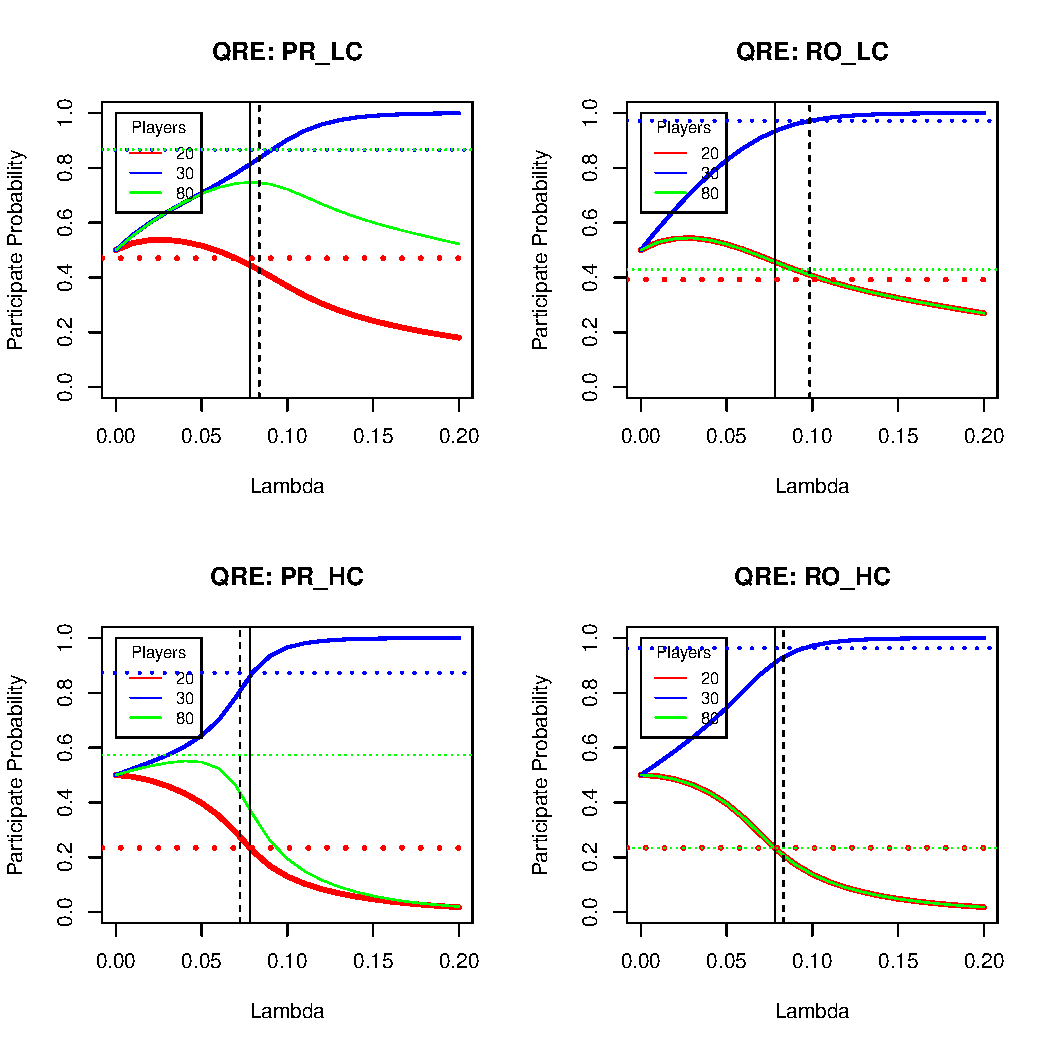
\includegraphics[width=1\linewidth]{../../results/figures/QRE_lambda_MLE}
		\caption{}
		\label{fig:qrelambdamle}
	\end{subfigure}
	\hfill
	\begin{subfigure}{0.7\textwidth}
		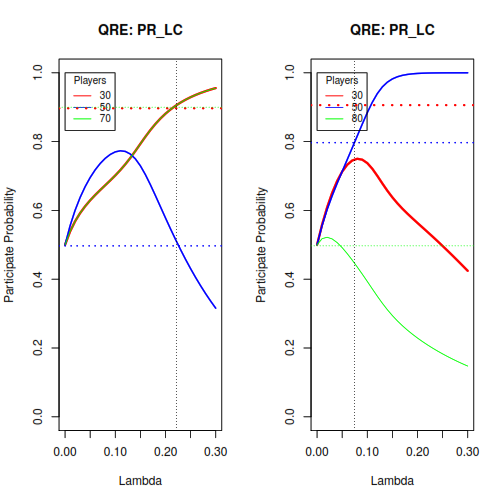
\includegraphics[width=0.6\linewidth]{../../results/figures/1st_treatments_plot}
		\caption{}
		\label{fig:1sttreatmentsplot}
	\end{subfigure}

\caption{QRE expected as a function of $\lambda$}
\label{fig:QRE}
\end{figure}


\subsubsection{Other Equilibria}

Other QRE emerge when $\lambda$ increase if there are other NE because they are especial cases of the QRE when $\lambda\rightarrow\infty$.
When $\lambda$ equals $0$ complete randomness is the only equilibrium, as can be seen in figure \ref{fig:qrelambdamle}. From this point, comes an equilibrium called \emph{logit equilibrium}\cite{Goeree2016}. 
Stochastic best responses seem continuous (even differentiable) functions of the parameter $\lambda$. However, as this parameters increases there will appear other equilibria from anywhere. 

Those equilibria can be seen in figures \ref{fig:ex70eqilibria} and \ref{fig:prlceqilibria}. It is seen as a discrete change in the probability of entry expected for each ideal point. Particularly, in figure \ref{fig:prlceqilibria}, we can see that equilibrium tended towards $q_{30}$ entering alone, and suddenly it is left out the election when $\lambda$ is around $0.15$. On the other hand, in figure \ref{fig:ex70eqilibria}, the contrary pattern is observed when $\lambda$ is around $0.17$.

\begin{figure}[h]
	\begin{subfigure}{0.5\textwidth}
		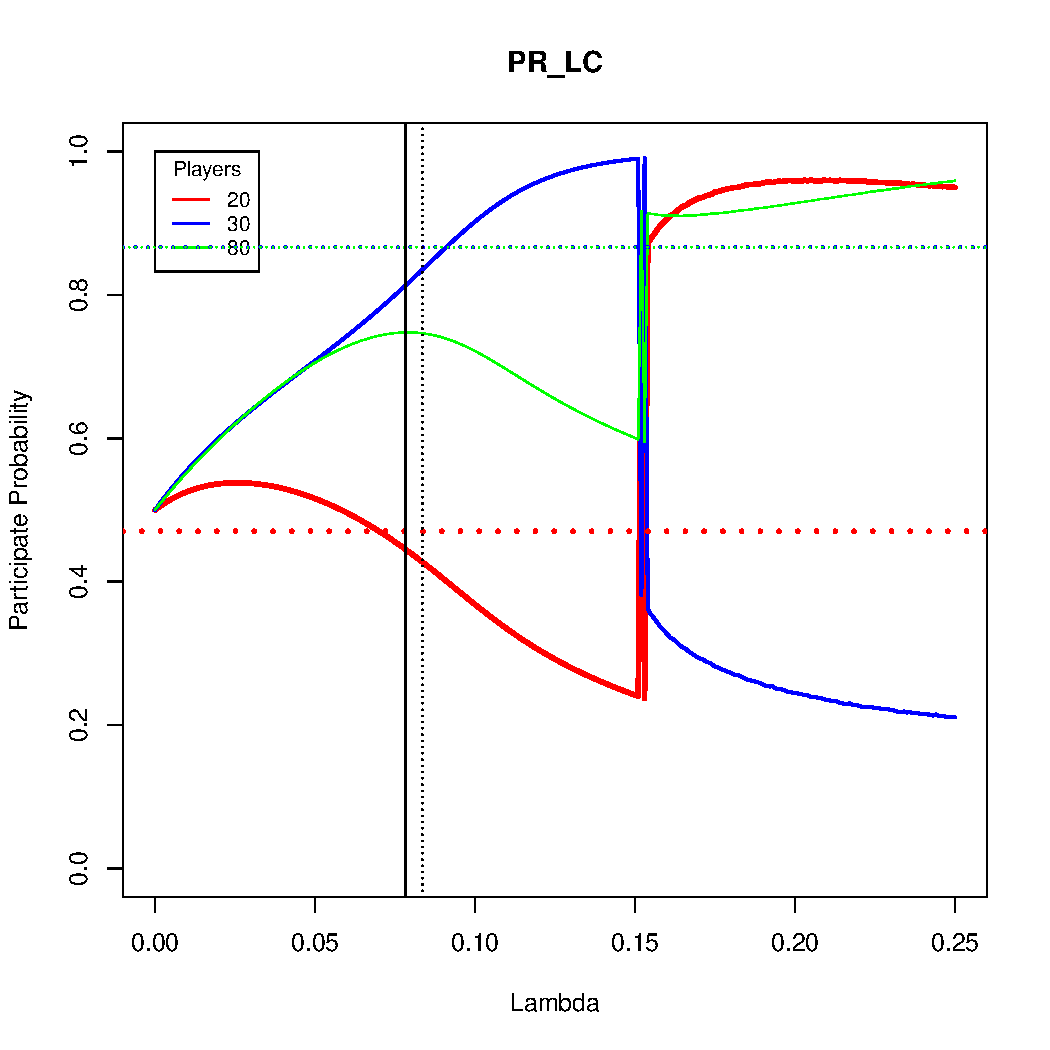
\includegraphics[width=0.7\linewidth]{../../results/figures/PR_LC_eqilibria}
		\caption{}
		\label{fig:prlceqilibria}
	\end{subfigure}
	\hfill
	\begin{subfigure}{0.5\textwidth}
		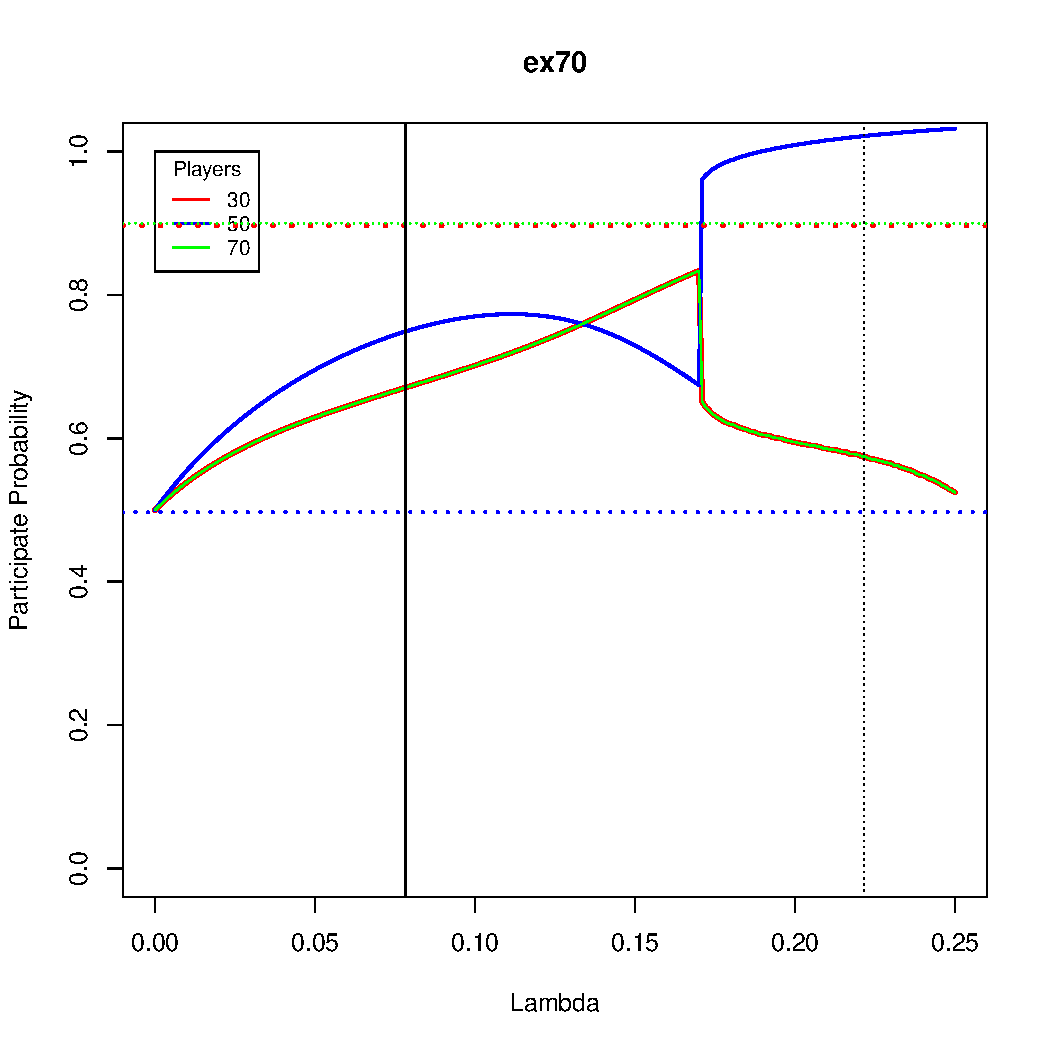
\includegraphics[width=0.7\linewidth]{../../results/figures/ex70_eqilibria}
		\caption{}
		\label{fig:ex70eqilibria}
	\end{subfigure}

\label{fig:otherQRE}
\caption{Other equilibrium that emerge when  $\lambda$ increases.}
\end{figure}


\section{Conclusion}

%Quantal response Equilibrium, which consider stochastic behavior, can describe candidates' decisions in the experiment. 

There is variability in the data that can not be explained by random error alone: there are systematic deviations from the standard prediction of NE that can be explained by QRE theory. This theory considers that participants' decisions depends stochasticity on the expected payoffs they face, which also depend on other's decisions that are also random. If we assume that players consider that others behave in the same way, QRE is the point when strategies and beliefs about strategies are the same.  

Considering that citizen-candidate assumption describe well enough the electoral process, the main prediction of QRE theory is that there are more candidates than expected by standard game theory. % review why there is not less entrance
This is the result of a direct and indirect effect of the stochastic best response. % check for direct and indirect effects of stocastic behavior as derivatives using calculus
First, there is a direct effect of the stochasticity that made the Nash winner ($q_{30}$) less probable to enter and increase the probability of others to enter. 
Second, others candidates increase their expected payoffs to participate because the probability of being defeated decreases relative to NE. % there could be the case of a reversal in a Nash winner strategy?, i.e. QRE for her gives a probability of less than 0.5 % review model of federesen specifically the case when there are many candidates at the median and one diferenciated one. In the present case review for the {20,80} equilibrium 
The magnitude of this indirect effect depends on the citizen's position relative to Nash winner; distant candidates to her are more prone to participate. This implication goes according with data observed.

Notice that the model adjust considerably good in al the experimental treatments when the parameter of stochasticity ($\lambda$) is calculated for those games. This parameter is similar in all games except for one where it is relatively higher. The reasons of this increase of $\lambda$ in this game are unclear. It is possible that it is related with the fact that game \textit{ex70} is the only game with an equilibrium where extreme ideal points enter in a higher proportion.

Finally, it most be noted that NE is not a bad forecasting. Nevertheless, QRE not just offer a more precise description, but also predict other interesting phenomena in data.

\bibliographystyle{apacite} 

\bibliography{library}

\end{document}
